\chapter{Recurrent models}
\label{chap:rnns}

\begin{supportbox}{About this chapter}
Transformer models are very effective at processing sequences, but they are hindered by their quadratic complexity in the sequence length. One possibility is to replace them with recurrent layers, having only constant-time for processing each element of a sequence, irrespective of its length. In this final chapter we provide an overview of several recurrent models and their characteristics. The field has been moving very rapidly in the last two years, and we provide a wide overview at the expense of precision -- see \cite{tiezzi2024state} for a recent survey.
\end{supportbox}

\section{Linearized attention models}
\subsection{Replacing the dot product}
\label{sec:linearized_transformer_model}

To provide some intuition on why recurrent neural networks (RNNs) can be useful, we begin with a generalization of the attention layer (called the \textbf{linearized attention layer} \cite{katharopoulos2020transformers}) that can be written in a recurrent form. We start by rewriting the SA layer in an abstract form with a generic scalar-valued attention function $\alpha(\cdot, \cdot)$ instead of the dot product:
%
\begin{equation}
\mathbf{h}_i=\frac{\sum_{j=1}^n\alpha\left(\mathbf{q}_i, \mathbf{k}_j\right)\mathbf{v}_j}{\sum_{j=1}^n \alpha\left(\mathbf{q}_i, \mathbf{k}_j\right)}
\label{eq:generalized_attention}
\end{equation}
%
where for the standard SA, $\alpha(\mathbf{x}, \mathbf{y})=\exp(\mathbf{x}^\top\mathbf{y})$. If the elements of the sequence must be processed in order (as in autoregressive generation), \eqref{eq:generalized_attention} is inconvenient because its cost grows quadratically in the sequence length. Even if a KV cache is used, memory still grows linearly. By comparison, a convolutional layer has fixed time and memory cost for each element to be processed, but information is lost if a token is outside the receptive field. What we would like, instead, is a mechanism to compress all the information of the sequence into a fixed-size input (which we will call a \textbf{memory} or \textbf{state} tensor), so that the cost of running the model on our current input token plus the memory is constant. We call models of this form \textbf{recurrent}.

To begin, note that any non-negative $\alpha$ is a valid similarity function. In machine learning, this requirement is equivalent to $\alpha$ being what is called a \textbf{kernel function} \cite{hofmann2008kernel}. Many such kernel functions can be written as a generalized dot product:
%
\begin{equation}
\alpha(\mathbf{x}, \mathbf{y})=\phi(\mathbf{x})^\top \phi(\mathbf{y})
\label{eq:kernel}
\end{equation}
%
for some function $\phi: \mathbb{R}^c \rightarrow \mathbb{R}^e$ that performs a feature expansion. 

\begin{supportbox}{Kernel functions}
As an example, the \textbf{polynomial kernel function} $\alpha(\mathbf{x}, \mathbf{y})=(1 + \mathbf{x}^\top\mathbf{y})^d$ can be rewritten as \eqref{eq:kernel} if $\phi(\bullet)$ explicitly computes all polynomials of its input up to order $d$ \cite{hofmann2008kernel}. Some kernel functions correspond to infinite-dimensional expansions (e.g., the Gaussian kernel), in which case (2) can still be recovered in terms of an approximated kernel expansion, such as working with random Fourier features \cite{scardapane2017randomness}.
\end{supportbox}
%
Based on \eqref{eq:kernel} we can rewrite \eqref{eq:generalized_attention} as:
%
$$
\mathbf{h}_i=\frac{\sum_{j=1}^n \phi(\mathbf{q}_i)^\top\phi(\mathbf{k}_j)\mathbf{v}_j^\top}{\sum_{j=1}^n \phi(\mathbf{q}_i)^\top\phi(\mathbf{k}_j)}
$$
%
where we have added a transpose operation on $\mathbf{v}_j$ to be consistent with the dimensions. Because $\phi(\mathbf{q}_i)$ does not depend on $j$ we can bring it outside the sum to obtain:
%
\begin{equation}
\mathbf{h}_i=\frac{{\color{drawred}\phi(\mathbf{q}_i)^\top}\sum_{j=1}^n \phi(\mathbf{k}_j)\mathbf{v}_j^\top}{{\color{drawred}\phi(\mathbf{q}_i)^\top}\sum_{j=1}^n \phi(\mathbf{k}_j)}
\label{eq:linearized_attention}
\end{equation}
%
This is called a \textbf{linearized attention} model \cite{katharopoulos2020transformers}. Computing \eqref{eq:linearized_attention} for all tokens has complexity $\mathcal{O}(n(e^2 + ev))$, which is linear in the sequence length and advantageous whenever $n <e^2$. $\phi$ can be chosen freely, e.g., in \cite{katharopoulos2020transformers} they consider a quadratic feature expansion or even a simpler $\phi(\mathbf{x})=\text{ELU}(\mathbf{x})+1$ for short sequences.

\subsection{A recurrent formulation}

We now rewrite the linearized attention model in a recurrent form, by considering what happens for a causal variant of the layer. First, we modify \eqref{eq:linearized_attention} by constraining the sum only on past input elements to make it causal:

\begin{equation}
\mathbf{h}_i=\frac{\phi(\mathbf{q}_i)^\top\eqnmarkbox[drawred]{node}{\sum_{j=1}^{\color{drawred}i} \phi(\mathbf{k}_j)\mathbf{v}_j^\top}}{\phi(\mathbf{q}_i)^\top\eqnmarkbox[drawgreen]{node2}{\sum_{j=1}^{\color{drawred}i} \phi(\mathbf{k}_j)}}
\label{eq:atf}
\end{equation}
\annotate[yshift=1em]{above,right}{node}{Attention memory $\mathbf{S}_i$}
\annotate[yshift=-1em]{below,right}{node2}{Normalizer memory $\mathbf{z}_i$}

\vspace{1em}
This is our first example of a \textbf{recurrent layer}. To understand the name, we note that the attention and normalizer memories can be written recursively as:
%
\begin{gather}
\mathbf{S}_i =\mathbf{S}_{i-1} + \phi(\mathbf{k}_i)\mathbf{v}_i^\top \label{eq:atf_recurrent_1} \\ 
\mathbf{z}_i = \mathbf{z}_{i-1}+\phi(\mathbf{k}_i) \label{eq:atf_recurrent_2}
\end{gather}
%
where the base case of the recurrence is given by their initialization:
%
\begin{gather}
\mathbf{S}_0=\mathbf{0} \\ \mathbf{z}_0=\mathbf{0}
\label{eq:atf_recurrent_init}
\end{gather}
%
The output is then given by:
%
\begin{gather}
\mathbf{h}_i=\frac{\phi(\mathbf{q}_i)^\top\mathbf{S}_i}{\phi(\mathbf{q}_i)^\top\mathbf{z}_i} \label{eq:atf_recurrent_3}
\end{gather}
%
Equations \eqref{eq:atf_recurrent_1}-\eqref{eq:atf_recurrent_3} are particularly interesting for an autoregressive scenario: for any new token to be generated, we update the two memory states (equations \eqref{eq:atf_recurrent_1} and \eqref{eq:atf_recurrent_2}), and we use these updated states to compute the output for the $i$-th element. Importantly, the total computation for generating a new token is constant, and the cost in memory is also fixed since the previous memories $\mathbf{S}_{i-1}$ and $\mathbf{z}_{i-1}$ can be discarded. We can alternate between the two formulations of the layer: we can use a vectorized variant for training (for efficient implementation on GPUs) and the recurrent formulation for inference. 

\section{Classical recurrent layers}
\subsection{General formulation}

\begin{SCfigure}
    \centering
    \hspace{2em}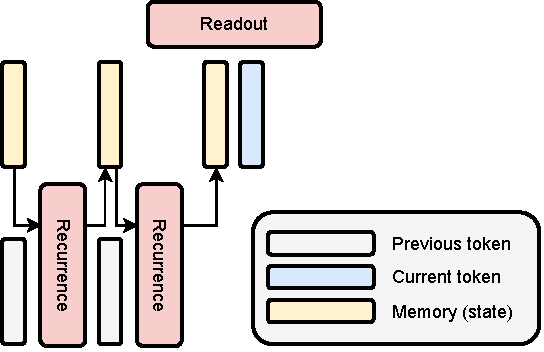
\includegraphics[width=0.5\textwidth]{images/recurrence}
    \caption{Overview of a recurrent layer: past tokens are shown in gray, current input token in blue, the memory state in yellow.}
    \label{fig:recurrence}
\end{SCfigure}

Let us now abstract away the key components of a recurrent layer, using the previous section as reference. First, we need a \textbf{state} of fixed size, which is used to compress all useful information up to the $i$-th element of the sequence. We denote it generically as $\mathbf{s}_i$, and without lack of generality we assume it is a single vector from now on. Second, we need a \textbf{transition function} (recurrence) that updates the state vector based on the previous value and the value of the current token, which we denote as $f(\mathbf{s}_{i-1}, \mathbf{x}_i)$. Third, we need what we call a \textbf{readout function} that provides an output for the $i$-th element of the sequence. We denote it as $g(\mathbf{s}_i, \mathbf{x}_i)$. See also Figure \ref{fig:recurrence} for a visualization. 

\begin{definition}[Recurrent layer] \addbottle
%
Given a sequence of tokens $\mathbf{x}_1, \mathbf{x}_2, \ldots$, a generic recurrent layer can be written as: 
%
\begin{gather}
\mathbf{s}_i = f(\mathbf{s}_{i-1},\mathbf{x}_i) \label{eq:recurrent_layer_state_update} \\ 
\mathbf{h}_i = g(\mathbf{s}_i, \mathbf{x}_i) \label{eq:recurrent_layer_readout}
\end{gather}
%
where the \textbf{state vector} $\mathbf{s}_i \sim (e)$ is initialized as zero by convention, $\mathbf{s}_0 = \mathbf{0}$. The size of the state vector, $e$, and the size of the output vector $\mathbf{h}_i \sim (o)$ are hyper-parameters. We call $f$ the \textbf{state transition} function and $g$ the \textbf{readout} function.
%
\end{definition}

%
In this format, a recurrent layer represents a discrete-time, input-driven dynamical system, and it is a causal layer by definition. In control engineering, this is also known as a \textbf{state-space model}. For tasks in which causality is unnecessary, \textbf{bidirectional layers} \cite{schuster1997bidirectional} can also be defined. In a bidirectional layer we initialize two recurrent layers (with separate parameters), one of which processes the sequence left-to-right, and the second one right-to-left. Their output states are then concatenated to provide the final output. 

Recurrent neural networks (RNNs) can be built by stacking multiple recurrent layers on the updated sequence $\mathbf{h}_1, \mathbf{h}_2, \ldots, \mathbf{h}_n$ \cite{pascanu2013construct}. Interestingly, a recurrent layer has no requirement on the length of the sequence, which can (in principle) be unbounded. For this reason, RNNs with unbounded precision or growing architectures can be shown to be Turing-complete \cite{chung2021turing}.

\begin{supportbox}{Implicit layers}
%
What happens if we apply a recurrent layers to a \textit{single} token $\mathbf{x}$?
%
\begin{equation}
\mathbf{s}_i = f(\mathbf{s}_{i-1}, \mathbf{x})
\label{eq:recurrent_layer_single_token}
\end{equation}
%
If we run the state transition several time starting from a known initialization $\mathbf{s}_0$, this is similar to a model with several layers (one per transition) sharing the same parameters. Suppose we run \eqref{eq:recurrent_layer_single_token} an \textit{infinite} number of times. If the dynamic system has a stable attractor, the output will be defined by the fixed-point equation:
%
\begin{equation}
\mathbf{s} = f(\mathbf{s}, \mathbf{x})
\label{eq:fixed_point_layer}
\end{equation}
%
If we take \eqref{eq:fixed_point_layer} as the definition of a layer, we obtain what is called an \textbf{implicit layer} \cite{bai2019deep}. The implementation of implicit layers can be made feasible by using fast solvers for the fixed-point equation and computing the backward pass with the use of the \textbf{implicit function theorem} \cite{bai2019deep}. Implicit graph layers can also be defined by running each diffusion operation to a stable state \cite{gori2005new,scarselli2008graph}. 
%
\end{supportbox}

\vspace{-0.5em}
\subsection{“Vanilla” recurrent layers} \addclock

Historically, recurrent layers were instantiated by considering two fully-connected layers as transition and readout functions:
%
\begin{gather}
f(\mathbf{s}_{i-1},\mathbf{x}_i)= \phi(\mathbf{A}\mathbf{s}_{i-1}+\mathbf{B}\mathbf{x}_i)\\g(\mathbf{s}_i,\mathbf{x}_i)=\mathbf{C}\mathbf{s}_i+\mathbf{D}\mathbf{x}_i
\end{gather}
%
where as always we ignore biases for simplicity, and we have four trainable matrices $\mathbf{A} \sim (e,e)$, $\mathbf{B} \sim (e,c)$, $\mathbf{C} \sim (o,e)$, and $\mathbf{D} \sim (o,c)$, where $c$ is the input dimensionality (the size of each token). A layer in this form is sometimes referred to generically as a “\textit{recurrent layer}”, a “\textit{vanilla recurrent layer}”, or an \textbf{Elman} recurrent layer. When the two matrices $\mathbf{A}$ and $\mathbf{B}$ are left untrained and we only have a single layer, these models are called \textbf{echo state networks} (ESNs) or \textbf{reservoir computers} \cite{lukovsevivcius2009reservoir}. ESNs can be a powerful baseline for time series forecasting, especially when the untrained matrices (the reservoir) are initialized in a proper way \cite{gauthier2021next}.

Despite their historical significance, layers of this form are extremely inefficient (and hard) to train. To see this, note that by its design the computation across elements of the sequence cannot be parallelized efficiently, as shown in Box \ref{code:recurrence}. Hence, we need to resort to iterative (for-loops) implementations, and even highly customized CUDA implementations\footnote{\url{https://docs.nvidia.com/deeplearning/performance/dl-performance-recurrent/index.html}} are slower than most alternative sequence layers. 

\begin{mypy}{Vanilla recurrence in PyTorch. It is impossible to parallelize the for-loop with linear algebra because of the dependencies in the recurrence. In PyTorch, the state update is called a \textbf{recurrent cell}, while the recurrent layers, such as {\footnotesize\mintinline{python}{torch.nn.RNN}}, wrap a cell and perform the complete for-loop.}{code:recurrence}
# Input tensor
x = torch.randn(batch_size, sequence_length, features)

# State tensor
s = torch.zeros(batch_size, state_size)

# State update
state_update = nn.RNNCell(features, state_size)
for i in range(x.shape[1]):
  s = state_update(x[:, i, :], s)
\end{mypy}

Another issue stems from the gradients involved in the layer’s computations. Consider a simplified case having only the transition function. We can unroll the full computation as:
%$
\begin{gather*}\mathbf{s}_1=f(\mathbf{s}_0,\mathbf{x}_1) \\ \mathbf{s}_2=f(\mathbf{s}_1,\mathbf{x}_2) \\ \vdots \\ \mathbf{s}_n=f(\mathbf{s}_{n-1},\mathbf{x}_n)\end{gather*}
%
This is similar to a model with $n$ layers, except that the parameters are shared (the same) across the layers. Below we focus on the quantity $\partial_{\mathbf{A}} \mathbf{s}_n$ (the weight Jacobian with respect to $\mathbf{A}$), but similar considerations apply to all gradients. Let us define the following cumulative product:
%
\begin{equation}\widetilde{\mathbf{s}}_i = \prod_{j={i+1}}^{n}\partial_{\mathbf{s}_{j-1} }f(\mathbf{s}_{j-1},\mathbf{x}_j)\end{equation}
%
This represents the gradient of the transition function from the end of the sequence backwards to element $i$, as shown in Figure \ref{fig:recurrence_backward}. Because of weight sharing, the gradient we are looking for has a separate term for each element in the sequence which involves these cumulative products:
%
\begin{equation} 
\partial_{\mathbf{A}} \mathbf{s}_n = \eqnmarkbox[drawred]{node}{\partial_{\mathbf{A}} f(\mathbf{s}_{n-1}, \mathbf{x}_n)} + \sum_{i=1}^{n-1}  \eqnmarkbox[drawgreen]{node2}{\widetilde{\mathbf{s}}_i \bigl[ \partial_{\mathbf{A}} f(\mathbf{s}_{i-1}, \mathbf{x}_i)\bigr]}
\label{eq:backpropagation_through_time}
\end{equation}
\annotate[yshift=-1em]{below,left}{node}{Gradient from element $n$}
\annotate[yshift=-1em]{below,right}{node2}{Gradient from element $i$}

\begin{SCfigure}
    \centering
    \hspace{2em}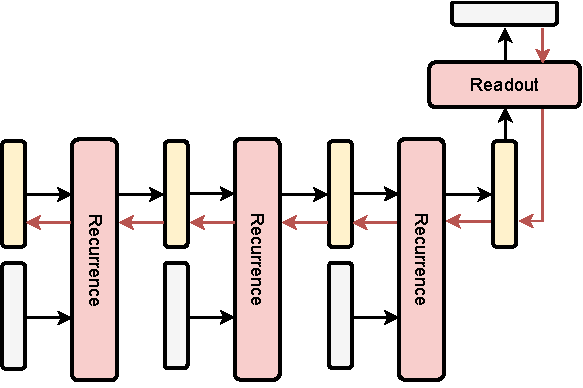
\includegraphics[width=0.5\textwidth]{images/recurrence-Pagina-2}
    \caption{Backward pass for a recurrent layer: the adjoint values have to be propagated through all the transition steps. Each state then contributes a single term to the full gradient of the parameters.}
    \label{fig:recurrence_backward}
\end{SCfigure}

The first term corresponds to a “standard” weight Jacobian, describing the influence of $\mathbf{A}$ on the last element of the sequence. The terms in the summation are the additional contributions, one for each element of the sequence, which are weighted by the chained input Jacobian computed over the sequence itself. 

Written in this form, reverse mode automatic differentiation is also called \textbf{backpropagation through time} (BPTT), and it can be a strong source of instability or gradient problems during gradient descent. To see this, note that each input Jacobian in the inner product in \eqref{eq:backpropagation_through_time} involves a multiplication by the derivative of the activation function $\phi$. Some of the earliest analyses of vanishing and exploding gradients were done in this context \cite{hochreiter1998recurrent}. For long sequences, stability of the layer is guaranteed only when the eigenvalues of the transition matrix are properly constrained \cite{gallicchio2017echo}. Layer normalization was also originally developed to stabilize training in RNNs, by computing statistics over the states’ sequence \cite{ba2016layer}.

Several techniques have been developed to partially solve these instabilities in the context of recurrent layers. For example, the sum in \eqref{eq:backpropagation_through_time} can be truncated to a given interval (\textbf{truncated BPTT}), or the gradients can be thresholded if they exceed a pre-defined upper bound (\textbf{clipped gradients}).

\subsection{Gated recurrent networks}

Over the years, several variants of the vanilla layer were proposed to improve its performance. In this section we focus on a popular class of such models, called \textbf{gated} RNNs. One issue of RNNs is that the entire state gets overwritten at each transition, which is reflected in the partial products in \eqref{eq:backpropagation_through_time}. However, we can assume that, for many sequences, only a few elements of these transitions are important: as an example, in an audio signal, empty regions or regions with no information are typical. In these cases, we may be interested in \textit{sparsifying} the transition (similarly to how most attention weights tend to be close to zero) and, consequently, setting most elements in $\widetilde{\mathbf{s}}_i$ to $1$. This can be achieved with the addition of specialized gating layers.

We consider the simplest form of gated RNN, called \textbf{light gated recurrent unit} (Li-GRU, \cite{ravanelli2018light}), having a single gate. For our purposes, a gating function is simply a layer that outputs values in the range $[0,1]$ that can be used to “mask” the input. As an example, a gate over the state can be obtained by a fully-connected layer with a sigmoid activation function:
%
$$
\gamma(\mathbf{s}_{i-1}, \mathbf{x}_i)=\sigma\left(\mathbf{V}\mathbf{s}_{i-1}+\mathbf{U}\mathbf{x}_i\right)
$$
%
where $\mathbf{V}$ and $\mathbf{U}$ have similar shapes to $\mathbf{A}$ and $\mathbf{B}$. We can interpret this as follows: if $\gamma_i \approx 0$, the $i$-th feature of the state should be kept untouched, while if $\gamma_1 \approx 1$, we should propagate its updated value as output. Hence, we can rewrite the transition function by properly masking the new and old values as:
%
$$
f(\mathbf{s}_{i-1}, \mathbf{x}_i) = \overbrace{\gamma(\mathbf{s}_{i-1}, \mathbf{x}_i)\odot\left(\mathbf{A}\mathbf{s}_{i-1}+\mathbf{B}\mathbf{x}_i\right)}^{\text{New values}} + \underbrace{(1-\gamma(\mathbf{s}_{i-1}, \mathbf{x}_i))\odot\mathbf{s}_{i-1}}_{\text{Old values}}
$$
%
This can be seen as a soft (differentiable) approximation to a “real” gate having only binary values, or as a convex combination of the original layer and a skip connection. We can theoretically control the goodness of this approximation by adding an additional regularizer to the loss that constrains the outputs of the gate to lie as close as possible to $0$ or $1$. 

Other gated recurrent layers can be obtained by adding additional gates to this design: the original  \textbf{gated recurrent unit} (GRU) adds a so-called “reset gate” to the layer \cite{cho2014learning}, while \textbf{long-short term memory} units (LSTMs) have a third “forget gate” \cite{hochreiter1997long}. LSTMs were the first gated variant to be introduced in the literature, and for a long time they have been the most successful deep architecture for processing sequences \cite{schmidhuber2015deep}. Because of this, research on LSTM models is still very active \cite{beck2024xlstm}.

\section{Structured state space models}
\subsection{Linear recurrent layers}

We now consider a simplified class of recurrent layers, in which we remove the intermediate nonlinearity in the transition function:
%
\begin{align}
f(\mathbf{s}_{i-1},\mathbf{x}_i)= \mathbf{A}\mathbf{s}_{i-1}+\mathbf{B}\mathbf{x}_i \label{eq:s4_1} \\
g(\mathbf{s}_i,\mathbf{x}_i)=\mathbf{C}\mathbf{s}_i+\mathbf{D}\mathbf{x}_i \label{eq:s4_2}
\end{align}
%
Written in this form, \eqref{eq:s4_1}-\eqref{eq:s4_2} are called \textbf{state space models} (SSM).\footnote{Confusingly, any recurrent layer in the form \eqref{eq:recurrent_layer_state_update}-\eqref{eq:recurrent_layer_readout} is an SSM, but in the neural network's literature the term SSM has come to be associated only with the linear variant. Sometimes we refer to them as \textbf{structured} SSMs because, as we will see, we need to properly constrain the transition matrix to make them effective.}  Intuitively, an SSM layer is “less expressive” than a standard recurrent layer (because of the lack of non-linearities). However, this can be recovered by adding activation functions after the output, or by interleaving these layers with token-wise MLPs \cite{orvieto2023universality}.

Interest in this class of models (re)-started in 2020, when \cite{gu2020hippo} analyzed a theoretical construction for the matrix $\mathbf{A}$ in \eqref{eq:s4_1} that could efficiently compress one-dimensional input sequences according to some pre-defined reconstruction criterion. The result was called the HiPPO (\textbf{High-Order Polynomial Projection Operator}) matrix. A family of neural networks built by a stack of SSM layers based on the HiPPO theory soon followed, leading to the \textbf{Structured State Space for Sequence Modeling} (S4) layer in 2021 \cite{gu2021efficiently} and the simplified S4 model (S5) in 2022 \cite{smith2022simplified}. 

Because of their roots in HiPPO theory, the proposed SSM layers up to S4 considered a stack of 1D models, one for each channel of the input, with transition matrices initialized as HiPPO matrices. By contrast, S5 introduced a standard multi-input, multi-output model of the form in \eqref{eq:s4_1}-\eqref{eq:s4_2}, which is the one we describe here. In particular, we focus our analysis on a simplified variant known as the \textbf{linear recurrent unit} (LRU) \cite{orvieto2023resurrecting}.

This formulation has a number of interesting properties, mostly stemming from the associativity of the linear transition function. To see this, we start by noting that the recurrence has a closed form solution:
%
\begin{equation}
\mathbf{s}_i =\sum_{j=1}^i\mathbf{A}^{i-j}\mathbf{B}\mathbf{x}_j
\end{equation}
%
We can view this summation from two different points of view. First, we can aggregate all coefficients with respect to the input sequence into a rank-3 tensor:
%
$$
K=\text{stack}\left( \mathbf{A}^{n-1}\mathbf{B}, \mathbf{A}^{n-2}\mathbf{B},\ldots,\mathbf{A}\mathbf{B},\mathbf{B}\right)
$$
%
We can compute all outputs via a single 1D convolution of filter size equal to the length of the sequence (a \textit{long} convolution) between the input sequence stacked into a single matrix $\mathbf{X} \sim (n,c)$ and the pre-computed kernel $K$:
%
$$
\mathbf{S}=\text{Conv1D}(\mathbf{X},K)
$$
%
Hence, the SSM layer can be interpreted as a convolution \cite{gu2021combining}. If the transition matrix is applied on a single channel, this can be exploited to speed-up computations by operating in a frequency domain, e.g., in the FlashConv implementation.\footnote{\url{https://www.together.ai/blog/h3}} However, a more efficient solution can be found by exploiting a family of algorithms known as \textbf{associative (parallel) scans} (or \textbf{all-prefix-sums}).

\subsection{An interlude: associative scans}

We introduce parallel scans in their general formulation before seeing their application to linear SSMs. Consider a sequence of elements $(x_1, x_2, \ldots, x_n)$, and an operation $\star$ which is assumed binary (it acts on any two elements of the sequence) and associative. We want to compute all partial applications of this operator to the sequence (using separate colors for readability):
%
$$
{\color{drawred_l}x_1}, \;\; {\color{drawgreen}x_1\star x_2}, \;\; {\color{drawblue}x_1\star x_2 \star x_3}, \;\; \ldots, \;\; x_1\star x_2 \star \cdots\star x_n
$$
%
This can be done trivially by an iterative algorithm which computes the elements one-by-one, adding one element at every iteration (this corresponds to how a standard recurrent layer would be computed). However, we can devise an efficient \textit{parallel} algorithm by exploiting the associativity of the operator $\star$ \cite{blelloch1990prefix}. The key intuition is that multiple pairs of elements can be computed in parallel and then aggregated recursively.

\begin{SCfigure}
    \centering
    \hspace{1em}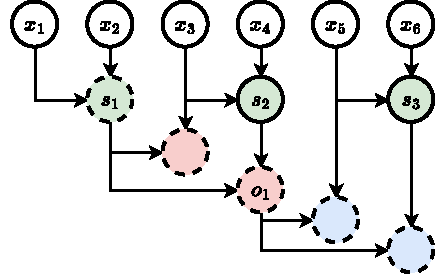
\includegraphics[width=0.45\textwidth]{images/associative_scan}
    \caption{Parallel scan on a sequence of six elements: circles of the same color can be computed in parallel; dashed circles are the outputs of the parallel scan.}
    \label{fig:associative_scan}
\end{SCfigure}

As a simple example, consider a sequence of 6 elements $x_1,x_2,x_3, x_4, x_5, x_6$ (an in-depth example applied to SSMs can be found in \cite{smith2022simplified}). We will denote by $\hat{x}_i$ the $i$-th prefix we want to compute. The overall procedure is shown schematically in Figure \ref{fig:associative_scan}. We first aggregate pairs of adjacent values as:
%
\begin{align*}
s_1 = x_1 \star x_2  & \rightarrow\hat{x}_2 \\s_2 = x_3 \star x_4 &\\ s_3 = x_5 \star x_6 &
\end{align*}
%
where we use arrows to denote output values of the algorithm. We now perform a second level of aggregations:
%
\begin{align*}
s_1 \star x_3 & \rightarrow \hat{x}_3 \\o_1 = s_1 \star s_2 & \rightarrow \hat{x}_4
\end{align*}
%
And finally:
%
\begin{align*} 
o_1 \star x_5 & \rightarrow \hat{x}_5 \\ o_1 \star s_3 & \rightarrow \hat{x}_6
\end{align*}
%
While this looks strange (we made 7 steps instead of 5), the three blocks of computations can be trivially parallelized if we have access to 3 separate threads. In general, by organizing the set of computations in a balanced fashion, we are able to compute the parallel scan in $\mathcal{O}(T \log n)$, where $T$ is the cost of the binary operator $\star$. An example of implementation is the associative scan function in JAX.\footnote{\url{https://jax.readthedocs.io/en/latest/_autosummary/jax.lax.associative_scan.html}}

It is easy to show that the transition function in a linear SSM is an example of an all-prefix-sums problem. We define the elements of our sequence as pairs $x_i = (\mathbf{A}, \mathbf{B}\mathbf{x}_i)$, and the binary operator as:
%
$$
(\mathbf{Z}, \mathbf{z})\star (\mathbf{V}, \mathbf{v})=(\mathbf{V}\mathbf{Z}, \mathbf{V}\mathbf{z}+\mathbf{v})
$$
%
The prefixes of $\star$ are then given by \cite{smith2022simplified}:
%
$$
x_1 \star x_2 \star \ldots \star x_i=(\mathbf{A}^i, \mathbf{s}_i)
$$
%
Hence, running a parallel scan gives us the powers of $\mathbf{A}$ as the first elements of the output, and all the states of the layer as the second element of the output. The complexity of this operation is upper bounded by the complexity of $\mathbf{A}^{i-1}\mathbf{A}$, which scales as $\mathcal{O}(n^3)$. To make the entire procedure viable, we can constrain $\mathbf{A}$ so that its powers can be computed more efficiently. This is the topic of the next section.

\subsection{Diagonal SSMs}

A common strategy to make the previous ideas feasible is to work with diagonal transition matrices (or diagonal matrices plus a low-rank term \cite{gu2021efficiently}). In this case, powers of $\mathbf{A}$ can be computed easily by taking powers of the diagonal entries in linear time. In addition, as we will see, working with diagonal matrices allows us to control the dynamics of the transition function to avoid numerical instabilities.

In particular, a square matrix $\mathbf{A}$ is said to be \textbf{diagonalizable} if we can find another square (invertible) matrix $\mathbf{P}$ and a diagonal matrix $\mathbf{\Lambda}$ such that:
%$
\begin{equation}
\mathbf{A} = \mathbf{P}\mathbf{\Lambda}\mathbf{P}^{-1}
\label{eq:diagonalizable_A}
\end{equation}
%
Diagonalizable matrices are (in a sense) “simpler” that generic matrices, For example, if such a decomposition exists, it is easy to show that powers can also be computed efficiently as:
%
$$
\mathbf{A}^i =\mathbf{P}\mathbf{\Lambda}^i\mathbf{P}^{-1}
$$
%
Suppose that the transition matrix is diagonalizable. Then, we can re-write the SSM in an equivalent form having a diagonal transition matrix. We begin by substituting \eqref{eq:diagonalizable_A} into the definition of the SSM and multiplying on both sides by $\mathbf{P}^{-1}$:
%
$$
\eqnmarkbox[drawred]{node}{\mathbf{P}^{-1}\mathbf{s}_i} =\sum_{j=1}^i\mathbf{\Lambda}^{i-j}\eqnmarkbox[drawgreen]{node2}{\mathbf{P}\mathbf{B}}\mathbf{x}_j
$$
\annotate[yshift=-1em]{below,left}{node}{New state vector $\bar{\mathbf{s}}_i$}
\annotate[yshift=-1em]{below,right}{node2}{New input-state matrix $\bar{\mathbf{B}}$}

We now rewrite the readout function in terms of the new variable $\bar{\mathbf{s}}$:
%
$$
\mathbf{y}_i = \eqnmarkbox[drawred]{node}{\mathbf{C}\mathbf{P}}\bar{\mathbf{s}}_i + \mathbf{D}\mathbf{x}_i
$$
\annotate[yshift=-1em]{below,right}{node}{New readout matrix $\bar{\mathbf{C}}$}

\vspace{-0.5em}
Putting everything together:
%
\begin{gather}
\bar{\mathbf{s}}_i=\mathbf{\Lambda}\bar{\mathbf{s}}_{i-1}+\bar{\mathbf{B}}\mathbf{x}_i \\ \mathbf{y}_i=\bar{\mathbf{C}}\bar{\mathbf{s}}_i+ \mathbf{D}\mathbf{x}_i
\end{gather}
%
Hence, whenever a diagonalization of $\mathbf{A}$ exists, we can always rewrite the SSM into an equivalent form having a diagonal transition matrix. In this case, we can directly train the four matrices $\mathbf{\Lambda} = \text{diag}(\lambda), \lambda \sim (e)$, $\bar{\mathbf{B}} \sim (e,c)$, $\bar{\mathbf{C}} \sim (o,e)$ and $\mathbf{D} \sim (o,c)$, with the diagonal matrix being parameterized by a single vector of dimension $e$.

Not all matrices can be diagonalized. However, an approximate diagonalization can always be found if one allows for matrices $\mathbf{P}$ and $\mathbf{\Lambda}$ to have complex-valued entries \cite{orvieto2023resurrecting}. Care must be taken to parameterize the values over the diagonal so that the eigenvalues of the transition matrix stay $< 1$ in absolute value, to avoid diverging dynamics. We refer to \cite{orvieto2023resurrecting} for a description of both points and for a complete analysis of the resulting LRU layer.

\vspace{-1em}
\section{Additional variants}
%
Balancing the different strengths of convolutions, recurrence, and attention is an active research topic. To close the book, we list some recurrent layers (or layers that can be interpreted as recurrent) that have been introduced very recently in the literature.
%
\subsection{Attention-free transformers}
%
One issue of the linearized transformer model (Section \ref{sec:linearized_transformer_model}) is the quadratic complexity in the feature dimension $e$. The attention-free transformer (ATF) was introduced as a variant of the basic attention layer that is instead linear in both sequence length and in the number of features \cite{zhai2021attention}.

The core idea is to replace the dot product interactions between keys, query, and values with a simpler \textit{multiplicative interaction} (element-wise):
%
\begin{equation}
\mathbf{h}_i=\sigma(\mathbf{q}_i) \odot\frac{\sum_j \exp\left(\mathbf{k}_j \right) \odot \mathbf{v}_j}{\sum_j\exp\left(\mathbf{k}_j \right)}
\label{eq:atf_new}
\end{equation}
%
This is similar to the self-attention layer, except that we replace all dot products with element-wise (Hadamard) multiplications. It is also inspired by the linearized attention layer in that the query is only used as a global modulation factor, in this case after normalizing it with a sigmoid operation. In fact, we can recover a standard attention formulation by rewriting \eqref{eq:atf_new} for a single dimension $z$ (exploiting the fact that we only perform element-wise operations):
%
$$
h_{iz}=\frac{\sigma(q_{iz})\sum_{j}\exp(k_{jz})}{\sum_j \exp(k_{jz})}v_{jz}
$$
%
Hence, the ATF layer can be re-interpreted as a channel-wise variant of attention, in the sense that for every channel we can rewrite it as an attention operation over the elements of the sequence. To increase flexibility, \cite{zhai2021attention} also considered adding relative embeddings $\mathbf{W} \sim (m, m)$ (where $m$ is the maximum allowed length of the sequences):
%
\begin{equation}\mathbf{h}_i=\sigma(\mathbf{q}_i) \odot\frac{\sum_j \exp\left(\mathbf{k}_j +W_{ij}\right) \odot \mathbf{v}_j}{\sum_j\exp\left(\mathbf{k}_j +W_{ij}\right)}\end{equation}

The relative embeddings can also be trained via a low-rank factorization to reduce the number of parameters. See \cite{zhai2021attention} for this and for additional variants of the basic ATF layer (e.g., hybridizing it with convolutional operations). We can also convert \eqref{eq:atf_new} to a causal (recurrent) variant by properly restricting the summation.

\subsection{The Receptance Weighted Key Value (RWKV) model}

The RWKV model \cite{peng2023rwkv} extends the ATF layer by incorporating a few additional architectural modifications. At the time of writing, this is one of the only pre-trained RNNs matching transformers at the largest scale, so we describe it in more detail. First, the relative embeddings are simplified by considering a single vector $\mathbf{w} \sim (e)$ which is scaled for each offset:
%
$$
w_{ij}=-(i-j)\mathbf{w}
$$
%
In addition, experiments showed that having a separate offset $\mathbf{u}$ (in place of $\mathbf{w})$ for the current element is beneficial. Written in causal form, this gives:

\begin{equation}
\mathbf{h}_i={\color{drawred}\mathbf{W}_o\Biggl(\Bigr.}\sigma(\mathbf{q}_i) \odot\frac{{\color{drawred}\sum_{j=1}^{i-1}}\exp\left(\mathbf{k}_j +w_{ij}\right) \odot \mathbf{v}_j{\color{drawred}+\exp\left(\mathbf{k}_i+\mathbf{u}\right) \odot \mathbf{v}_i}}{{\color{drawred}\sum_{j=1}^{i-1}}\exp\left(\mathbf{k}_j +w_{ij}\right){\color{drawred}+\exp\left(\mathbf{k}_i+\mathbf{u}\right)}}{\color{drawred}\Bigl.\Biggr)}
\label{eq:rwkv}
\end{equation}

where we highlight the differences from the basic ATF layer in red. The query is called the \textbf{receptance} in \cite{peng2023rwkv}, and an additional output projection $\mathbf{W}_o$ is added at the end. Second, the RWKV model modifies the standard MLP in the transformer block with a differently \textit{gated} token-wise block. For a given input token $\mathbf{x}$ this can be written as:
%
\begin{equation}\mathbf{y}=\sigma(\mathbf{W}_1\mathbf{x})\odot \mathbf{W}_2\max(0, \mathbf{W}_3\mathbf{x})^2\end{equation}

where $\mathbf{W}_1$, $\mathbf{W}_2$, and $\mathbf{W}_3$ are trainable parameters. This is a standard MLP except for the left-most gate and the use of the squared ReLU. As a final modification, all three projections in the first block (and also the two appearances of $\mathbf{x}$ in \eqref{eq:rwkv}) are replaced with convex combinations of $\mathbf{x}_i$ and $\mathbf{x}_{i-1}$ to improve performance, which is called \textit{token shift}.

\subsection{Selective state space models}

We have seen three classes of recurrent models: standard recurrent layers (and their gated versions), linearized attention layers, and structured state space models. Although they look different, it is relatively easy to move from one class of models to the other. To see this, let us consider a linearized attention layer where we ignore the denominator:
%
\begin{align}
\mathbf{S}_i=\mathbf{S}_{i-1}+\phi(\mathbf{k}_i)\mathbf{v}_i^\top \label{eq:lin_att_simplified_1} \\ \mathbf{h}_i=\phi(\mathbf{q}_i)^\top\mathbf{S}_i
\label{eq:lin_att_simplified_2}\end{align}
%
Apart from the matrix-valued state, we see this has the form of a SSM layer, except that some matrices (e.g., $\mathbf{C} = \phi(\mathbf{q}_i)^\top$) are not fixed but they depend on the specific input token. From the point of view of dynamic systems, we say that standard SSMs describe \textit{time-invariant} systems, while \eqref{eq:lin_att_simplified_1}-\eqref{eq:lin_att_simplified_2} describe a \textit{time-varying} system. This has inspired another class of SSM layers whose matrices are not constrained to be time-invariant, which have been called \textbf{selective} SSMs. Most of these models leverage the idea of attention layers of projecting the input multiple times before the layer’s computations.

\begin{SCfigure}
    \centering
    \hspace{2em}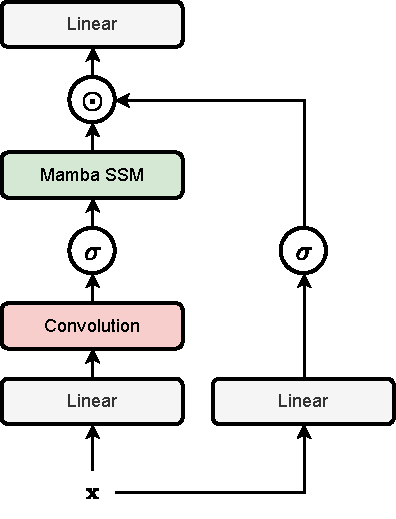
\includegraphics[width=0.4\textwidth]{images/mamba}
    \caption{Mamba block (residual connections around the block and normalization are not shown). $\sigma$ is the sigmoid function. Adapted from \cite{gu2023mamba}.}
    \label{fig:mamba}
\end{SCfigure}

As an example, we focus here on the so-called Mamba layer \cite{gu2023mamba} which, at the time of writing, is one of the few SSM layers that was scaled to match the performance of transformer models at very large contexts and parameters’ counts. First, in order to make the SSM layer time-varying, a subset of its matrices are made input-dependent:\footnote{The matrix $\mathbf{D}$ can be seen as a simple residual connection and it is left untouched. The original layer has a slightly different parameterization where $\mathbf{A} = \exp(\Delta \bar{\mathbf{A}})$, for some trainable $\bar{\mathbf{A}}$ and input-dependent scalar value $\Delta$. This does not change our discussion.}
%
\begin{gather}
\mathbf{s}_i = A(\mathbf{x}_i)\mathbf{s}_{i-1} + B(\mathbf{x}_i)\mathbf{x}_i \\ \mathbf{h}_i = C(\mathbf{x}_i)\mathbf{s}_i + \mathbf{D}\mathbf{x}_i 
\end{gather}
%
where $A(\bullet)$, $B(\bullet)$, and $C(\bullet)$ are linear projections of their input tokens. To make this feasible, the layer is applied to each channel of the input independently, and the transition  matrix is selected as diagonal, so that all matrices of the SSM can be represented with a single vector of values. This layer looses a simple parallel scan implementation and requires a customized hardware-aware implementation \cite{gu2023mamba}. It can be shown that the Mamba SSM variant and several other SSM layers are degenerate case of a gated recurrent layer \cite{gu2021combining,gu2023mamba}.

To make the overall architecture simpler, Mamba avoids alternating MLPs and SSMs, in favour of a gated archicture (similar to the gated attention unit from Section \ref{subsec:mha_variants}) where an MLP is used to weight the outputs from the SSM. An additional depthwise convolution is added for improved flexibility - see Figure \ref{fig:mamba}.